
%----------------------------------------------------------------------------------------
%	PACKAGES AND OTHER DOCUMENT CONFIGURATIONS
%----------------------------------------------------------------------------------------

\documentclass[fleqn,10pt]{SelfArx} % Document font size and equations flushed left

\usepackage[utf8]{inputenc}
\usepackage[T1]{fontenc}
\usepackage[english,spanish]{babel}

\usepackage{lipsum} % Required to insert dummy text. To be removed otherwise

%----------------------------------------------------------------------------------------
%	COLUMNS
%----------------------------------------------------------------------------------------

\setlength{\columnsep}{0.55cm} % Distance between the two columns of text
\setlength{\fboxrule}{0.75pt} % Width of the border around the abstract

%----------------------------------------------------------------------------------------
%	COLORS
%----------------------------------------------------------------------------------------

\definecolor{color1}{RGB}{0,0,90} % Color of the article title and sections
\definecolor{color2}{RGB}{0,20,20} % Color of the boxes behind the abstract and headings

%----------------------------------------------------------------------------------------
%	HYPERLINKS
%----------------------------------------------------------------------------------------

\usepackage{hyperref} % Required for hyperlinks
\hypersetup{hidelinks,colorlinks,breaklinks=true,urlcolor=color2,citecolor=color1,linkcolor=color1,bookmarksopen=false,pdftitle={Title},pdfauthor={Author}}

% Separación de elementos en itemize
\usepackage{enumitem}
\setlist{noitemsep}

%----------------------------------------------------------------------------------------
%	ARTICLE INFORMATION
%----------------------------------------------------------------------------------------

\JournalInfo{2016} % Journal information
\Archive{Minería de Datos, bajo la supervisión de la ingeniera Alexandra Pomares} % Additional notes (e.g. copyright, DOI, review/research article)

\PaperTitle{ESTUDIO SOBRE LA DESERCIÓN ESCOLAR UTILIZANDO MINERÍA DE DATOS EN LA MODALIDAD DE ENSEÑANZA VIRTUAL EN LA INSTITUCIÓN UNIVERSITARIA POLITÉCNICO GRANCOLOMBIANO} % Article title

\Authors{Jhonny Cano, Julian Olarte, Henry Solarte} % Authors
\affiliation{\textsuperscript{1}\textit{Universidad Politécnico Grancolombiano, Maestría en Ingeniería de Sistemas, Bogotá, Colombia}} % Author affiliation
%\affiliation{\textsuperscript{2}\textit{Universidad Politécnico Grancolombiano, Maestría en Ingeniería de Sistemas, Bogotá, Colombia}} % Author affiliation
\affiliation{*\textbf{Correos de los autores}: jhonnycano@hotmail.com, jolarter@poligran.edu.co, henrysolarte@hotmail.com} % Corresponding author

\Keywords{Modalidad Virtual --- Deserción --- Vista Minable} % Keywords - if you don't want any simply remove all the text between the curly brackets
\newcommand{\keywordname}{Keywords} % Defines the keywords heading name

%----------------------------------------------------------------------------------------
%	ABSTRACT
%----------------------------------------------------------------------------------------

\Abstract{En la actualidad la Institución Universitaria Politécnico Grancolombiano, oferta programas académicos a través de modalidad virtual, en esta modalidad de enseñanza hay una elevada tasa de deserción estudiantil; en este proyecto se utiliza la minería de datos como herramienta fundamental que puede contribuir a determinar las causas de deserción con el fin de adoptar mecanismos que disminuyan este fenómeno. Para lograr este objetivo se cuenta con diversos orígenes de datos suministrados por el claustro universitario, los cuales se depuran y preparan para su posterior utilización en una vista minable y luego se procesan mediante un aplicativo llamado RapidMiner. Los hallazgos encontrados arrojan causales comunes que llevan a la deserción estudiantil en modalidad virtual y brindan conocimiento básico y fundamental con miras a instituir procesos que eviten la deserción.}

%----------------------------------------------------------------------------------------

\begin{document}

\flushbottom % Makes all text pages the same height

\maketitle % Print the title and abstract box

\tableofcontents % Print the contents section

\thispagestyle{empty} % Removes page numbering from the first page

%----------------------------------------------------------------------------------------
%	ARTICLE CONTENTS
%----------------------------------------------------------------------------------------

\section*{Introducción} % The \section*{} command stops section numbering

\addcontentsline{toc}{section}{Introducción} % Adds this section to the table of contents
La Universidad Politécnico Grancolombiano tiene como misión ofrecer educación con altos estándares de calidad a la sociedad colombiana, y de este modo contribuir a su cualificación y crecimiento.\\

Por este motivo, y con miras de llegar a la mayor parte del territorio de nuestro país, la Universidad ha incursionado en el mercado educacional a través de la modalidad virtual.\\

No obstante lo anterior, dentro de esta modalidad académica existe un alto número de deserciones, lo cual se traduce en una disminución de conocimiento y personal capacitado en el país.\\

En este contexto, la Ingeniería de Sistemas puede suministrar herramientas valiosas que permitan a esta comunidad académica conocer las causales que originan el fenómeno de la deserción, con el fin de adoptar las medidas necesarias para disminuir esta problemática.\\

La minería de datos entonces se vislumbra como una herramienta material y efectiva que nos permite lograr este cometido por medio de un proceso claramente definido, cuyo resultado final contribuirá a entender el fenómeno y promover acciones para su erradicación.

En dicho proceso existen diversas tareas que nos permiten realizar la transición de los datos en información y éste en conocimiento.

Entre las primeras tareas se encuentra la comprensión tanto del negocio, como de los datos con los que se cuenta para realizar la tarea de minería, esto con el fin de plantear los objetivos a los que se quiere llegar por medio del proyecto de minería de datos, y cómo se traduce este objetivo de minería en un objetivo de negocio.

Luego de entender los datos disponibles, se debe proceder a una fase de preparación de los mismos, con el fin de que se ajusten a las entradas requeridas por los algoritmos de minería identificados como factibles de aplicar en las fases iniciales del proyecto.

Posteriormente, en la fase de modelado, se procesan y calibran los parámetros de los modelos para extraer los mejores resultados a partir de los algoritmos elegidos.

Existen otras fases posteriores, que permiten evaluar el resultado del proyecto de minería y generalizar su aplicación dentro de la organización.

%------------------------------------------------

\section{Trabajos Relacionados}
Respecto al tema objeto de investigación, se han adelantado varios estudios, entre los cuales destacan:\\

La investigación efectuada por Márquez, Romero y Ventura en la Unidad Académica Preparatoria de la Universidad Autónoma de Zacatecas (UAPUAZ) de México, investigación que acude a la minería de datos para analizar el fenómeno de la deserción universitaria. Se ha mostrado la utilidad de las técnicas de selección de características al utilizar un conjunto reducido de 15 atributos de entre los 77 disponibles inicialmente, se han seleccionado 10 algoritmos de clasificación disponibles por la herramienta de minería de datos Weka, obteniendo un modelo de salida comprensible para el usuario, y se obtienen reglas de clasificación del tipo “Si – Entonces” o árboles de decisión.\\

A su vez, la Universidad de la Sabana por conducto de Maria Claudia Moreno y Stephanie Mendez, acudió a la minería de datos con el fin de realizar un estudio de deserción universitaria en la facultad de ingeniería. En esta investigación se aplicó la metodología \textit{Rough set}, que busca la identificación de las variables criticas influyentes.\\

En la Universidad de Nariño, los investigadores Ricardo Timarán Pereira, Andrés Calderón Romero, Javier Jiménez Toledo, adelantaron una investigación sobre el descubrimiento de perfiles de deserción estudiantil con técnicas de minería de datos. Dentro de la misma se recurrió a las técnicas de clasificación y clustering sobre los datos de los estudiantes utilizando el aplicativo Weka.\\


%------------------------------------------------

\section{Justificación}

El Ministerio de Educación Nacional, define la deserción como una situación a la que se enfrenta un estudiante cuando aspira y no logra concluir su proyecto educativo, considerándose como desertor a aquel individuo, que siendo estudiante de una institución de educación superior, no presenta actividad académica durante dos semestres académicos consecutivos, lo cual equivale a un año de inactividad académica. \\

La educación Superior en Colombia presenta altas tasas de deserción estudiantil, especialmente en los primeros semestres académicos, lo cual conlleva a efectos de tipo financiero, académico y social, tanto para las Instituciones de Educación Superior (IES) como para el estudiante, la región, y el país. \\

La Institución Universitaria Politécnico Grancolombiano, no es ajena a esta situación, toda vez que en la modalidad de educación virtual ofertada por este claustro universitario, se presenta en gran volumen deserción estudiantil, generando disminución de cobertura y de la materialización del quehacer institucional.\\

En este contexto es de vital importancia analizar las causas que originan esta problemática, esto, con la finalidad última de lograr disminución de estas tasas y así contribuir a la cualificación y progresión del estado, ya que al incrementar la población profesional de una nación, se crea desarrollo progreso y avances en las diferentes esferas que la conforman, lo que genera altos niveles de crecimiento y tecnificación.\\

Ahora bien, la Ingeniería de Sistemas, a través de áreas como la minería de datos, permite realizar investigaciones que arrojan información sobre las causas que originan deserción, lo cual se traduce en un insumo vital que permite adoptar estrategias, medidas y acciones, que inciden de forma directa y efectiva en la prevención de la deserción estudiantil.\\

Esto a su vez, permite mitigar este fenómeno derivando en un proceso académico sostenible y reduciendo afectaciones que van desde la órbita económica hasta la sociocultural.\\


%------------------------------------------------
%\phantomsection
\section{Procedimiento}

El Politécnico Grancolombiano recibe cada semestre un número significativo de estudiantes en sus programas académicos en modalidad presencial y virtual. 
La tasa de permanencia de los estudiantes y su continuidad en esta institución, se calcula sobre las matrículas recibidas en cada semestre, versus las matrículas recibidas en el semestre anterior. A su vez, el complemento del indicador permanencia es el indicador de deserción, que presenta los siguientes datos históricos para los últimos cuatro años (siete periodos):  \\

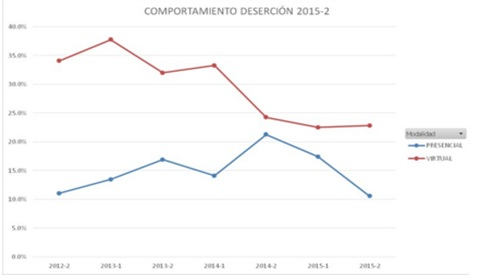
\includegraphics[width=8cm]{img/estadistica.jpg}\\ 

Se espera que con este proyecto de minería de datos se identifiquen atributos, reglas o agrupaciones naturales de los estudiantes que toman la decisión de retirarse de un programa académico y crear programas, campañas y en general decisiones que desestimulen la deserción. \\

Por tanto, se requiere realizar una caracterización de los estudiantes para comprender el fenómeno de deserción y posteriormente se pretende crear un modelo que permita identificar los estudiantes que están en riesgo de desertar de un programa académico. Para delimitar el problema, se estudiarán únicamente los estudiantes de la modalidad virtual y su fenómeno de deserción durante los dos primeros semestres. \\
Gracias a la información suministrada por el Politécnico Grancolombiano, se procesaron seis tablas principales de las cuales se derivó el trabajo de investigación.\\

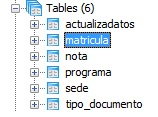
\includegraphics[scale=1]{img/tablas.jpg}  
%\addcontentsline{toc}{section}{Acknowledgments} % Adds this section to the table of contents

%So long and thanks for all the fish \cite{Figueredo:2009dg}.
Tabla {\bf ACTUALIZADATOS}, tiene información sobre los estudiantes que actualizaron su información personal en el año 2015. Cuenta con un total de 99.549 registros y 27 columnas. \\
Tabla {\bf NOTA} posee información de las notas de los estudiantes desde el año 2008. Esta tabla contiene un total de 867.011 registros y 32 columnas. \\
Tabla {\bf MATRICULA}, base de datos de las transacciones de matrícula, renovaciones, cambios de jornada, entre otros desde el 2003. \\
Información secundaria empleada en la investigación fue accesada de las tablas: Programa, sede, TipoDocumento.\\
Tabla {\bf PROGRAMA}, contiene información de los programas de la institución universitaria Politécnico Grancolombiano, con un total de 99 registros y un total de 7 columnas. \\
Tabla {\bf SEDE} con un total de 149 registros y un total de 5 columnas. \\
Tabla {\bf TIPO\_DOCUMENTO } con un total de 12 registros y un total de 2 columnas. \\

El análisis de calidad de datos se realiza una vez migrados los archivos de Excel a la base de datos de Postgres; previo a este análisis, se realizó reformateo de los nombres de las columnas para facilitar su trabajo con las mismas. A continuación se procede a verificar la consistencia de los campos, se tratará de realizar diferentes procedimientos en aquellos campos que no estén totalmente diligenciados, en caso de que no se pueda lograr su consistencia se procederá a eliminarlos. \\

De forma posterior, se procedió a almacenar la base de datos en un servidor de Amazon y un proveedor de Cloud llamado Heroku. Se precisa que Heroku es una plataforma de servicio de computación en la Nube que soporta distintos lenguajes de programación (php, Ruby, Python, etc.) y bases de datos (Postgres, MySql, etc.)\\

El objetivo de colocar la base de datos en la nube es permitir que las personas del grupo puedan trabajar con datos en tiempo real, y así dividir el trabajo en 3 Partes:\\
1.	Tabla Estudiantes, en donde cada estudiante fuera único, determinando ciertos atributos para esta tabla.\\
2.	Tabla  HistoricoMatriculas para conocer el comportamiento de los estudiantes respecto a las matrículas.\\
3.	Tabla de Nota para conocer el comportamiento de las notas de los estudiantes y su incidencia en la deserción.\\ 

Es así como se pasó de 6 tablas inicialmente a un total de 11 tablas, cifra última con la cual se desarrolló el trabajo.\\

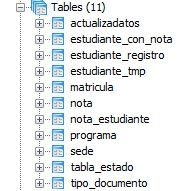
\includegraphics[width=4cm]{img/tablas11.jpg}\\ 

\subsection{Extracción de datos para estudiantes}

Una de las primeras tareas detectadas en la depuración de los datos consiste en adaptar los datos de estudiantes, de modo que quede una tabla donde cada registro represente un único estudiante. Para llegar a este resultado se realizaron los siguientes pasos:\\

\begin{itemize}
	\item Se extrajeron datos de estudiante de las diferentes tablas relacionadas (actualizadatos, matricula)
	\item Se cruzaron de modo que se pudiese acceder a una llave primaria con significado para el negocio (codigo\_estudiante)
	\item Se agruparon los datos para evitar la repetición de estudiantes.
	\item Una vez encontrada la tabla de estudiante, se verificó que no hayan estudiantes repetidos.
\end{itemize}

Al realizar la agrupación de datos, se detectó que el estudiante se repetía, con los mismos datos, pero con diferentes jornadas o sedes, esto ocurre porque un estudiante puede encontrarse inscrito en programas como inglés virtual, alianza con el SENA, etc., adicional a los programas convencionales.\\

Para poder individualizar esta información, se realizó el proceso similar a la numeración 1-n con miras a extraer información de filas a columnas para los atributos considerados como más importantes para la vista minable.

Así pues, los campos resultantes derivaron en:\\

\textbullet \ Jornada\_virtual \\ 
\textbullet \ Sedesena\_virtual\\
\textbullet \ Sede\_ingles\_virtual\\
\textbullet \ Sede\_pregrado\_virtual\\
\textbullet \ Sede\_postgrado\_virtual\\

\subsection{Extracción de datos para notas}

La tabla nota discutida en apartados anteriores, contiene un registro por cada nota definitiva de un estudiante en una materia determinada, relacionando además atributos como la carrera, la nota, el programa, entre otros; hubiese sido interesante contar con la información del profesor que dictó la materia, pero dadas las restricciones de tiempo, no fue posible acceder a dicha información.\\

Dado que para la vista minable la decisión fue que cada registro representase a un estudiante, esta información de notas debió ser manejada en agrupaciones para poder asociarla a un estudiante y que la misma fuera accedida en un solo registro; por tanto, se tomó la decisión de extraer la información de notas de los tres primeros periodos de cada estudiante, y para cada periodo.\\

Para extraer esta información, se siguió el procedimiento descrito a continuación:

En primer término, se individualizaron los registros de la tabla nota (tabla origen de las notas) por medio de una consulta GROUP BY; los datos de agrupación se crearon, dejando vacíos para calcular en pasos posteriores.\\

Para el segundo paso, se tomó el identificador de los primeros tres periodos para cada estudiante (campos s1\_id, s2\_id, s3\_id); en caso que no lo estuviera, también era importante marcar dicho identificador como NULL;

\section{Vista Minable}

Una vez culminada la fase de extracción de datos para estudiantes, extracción de datos para notas y extracción de datos para matriculas, se creó una tabla que contiene la vista minable, esta tabla se llamó vista\_minable\_clustering y cuenta con un total de 38 campos que son indispensables para el estudio en relación.\\

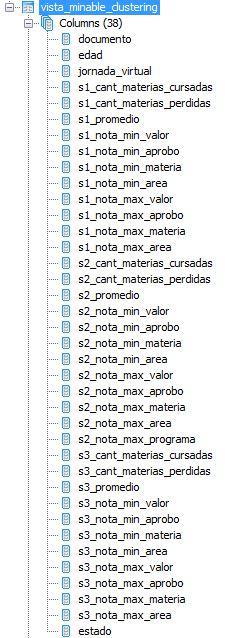
\includegraphics[width=3cm]{img/captura.jpg}\\ 
\\

\subsection{Síntesis de los ejercicios de minería de datos} 

Una vez obtenida la vista minable a partir de los datos a analizar, se procede a hacer los siguientes ejercicios:\\
\textbullet\ Separación de desertores según el periodo en el que desertaron.\\
\textbullet\ Generación de orígenes de datos para los diferentes ejercicios\\
\textbullet\ Preparación de datos para Clustering\\
\textbullet\ Conclusiones preliminares\\
\\
En la vista minable del anterior ejercicio, se obtuvo una cantidad de 4390 registros con clase "desertor", los cuales en algunas columnas tienen valores nulos, dependiendo del semestre en el que abandonaron sus estudios. Para poder manejar esta situación, se realizó una separación de desertores de acuerdo al último periodo en el cual tuvieran notas registradas. De este modo, se filtró la vista minable del ejercicio inicial en tres consultas:\\

\textbullet\ Desertores de primer semestre: Estudiantes marcados como "desertor" que no registraron notas en segundo semestre (1157).\\
\textbullet\ Desertores de segundo semestre: Estudiantes marcados como "desertor" que registraron notas en segundo semestre, pero no en tercer semestre (670).\\
\textbullet\ Desertores de tercer semestre: Estudiantes marcados como "desertor" que registraron notas en tercer semestre (2563).\\

De cada consulta, solamente se extrajeron los datos relevantes, de forma tal que las columnas que tenían valores NULL quedaron excluidas de cada análisis.\\

Para cada grupo de desertores, se realizó el ejercicio de clustering como se puede observar en la siguiente figura:

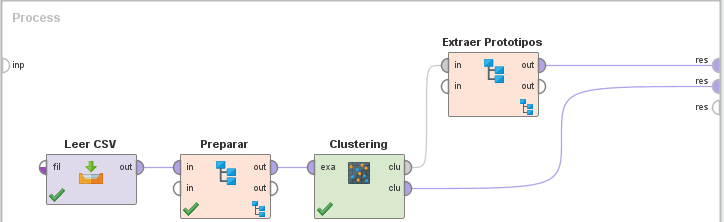
\includegraphics[width=8cm]{img/proc.png}\\ 

Como se puede apreciar, la primera tarea consiste en la lectura de datos desde un archivo csv extraído desde Postgres, para luego realizar las preparaciones de datos que se explicarán en secciones siguientes, y luego someter los datos transformados al algoritmo de clustering y como medida final, el almacenamiento del resultado detallado y de prototipos detectados en archivos de Excel; en las siguientes secciones se realiza una revisión del proceso de preparación realizado.

\subsection{Clustering de desertores en primer semestre}

Una vez extraídos los datos de desertores de primer semestre, se realizó una preparación de datos con el objetivo de exponer los datos a un algoritmo de clustering (k-means) que nos permitiera detectar patrones de similaridad o equivalencia en aquellos estudiantes.\\

Las siguientes fueron las tareas realizadas durante la preparación de datos:\\

\textbullet\ {\bf Exclusión de columnas (Materia)\\}

Debido a que hay muchas materias en esta vista, y teniendo en cuenta que la misma información se encuentra de forma agrupada en la variable "área", se decide excluir la columna de materia para facilitar los ejercicios sub-siguientes; esta decisión se sustenta realizando el primer ejercicio de clustering (desertores en primer periodo) sin encontrar diferencias sustanciales en los clustering resultantes.\\

\textbullet\ {\bf Materia y área (Nominal to Numerical)\\}

Para convertir la variable "área" en valores compatibles con el algoritmo de clustering, se realizó una numerización 1-n; al ver que hay relación entre las variables de materia y área, se decidió realizar el ejercicio de clustering dos veces, la primera vez usando la variable "materia" y la segunda vez, prescindiendo de ella para ver si se encontraban grupos más definidos de esta manera; como se explicó anteriormente, al hacer el ejercicio completo, no se encontraron grandes diferencias en los clusters encontrados, por lo que se decide proseguir con los demás ejercicios prescindiendo de la variable materia.\\

\textbullet\ {\bf Edad (Discretize y Nominal to Numerical)\\}

Para no usar la edad como un argumento entero, se discretizó este valor en diferentes categorías (0-18, 19-21, 22-24, 25-27, 28-30, 31-33, 33+).\\

Luego, estos valores fueron transformados en columnas (numerización) para poder someterlos al algoritmo de clustering.\\

\textbullet\ {\bf Valores numéricos (Normalize)\\}

Las variables restantes fueron normalizadas en rango 0-1: materias cursadas y perdidas, nota mínima y máxima, promedio.\\

Para este primer ejercicio de clustering, se encontraron varios clusters que inicialmente no nos brindaron información evidente; sin embargo, después de una cuidadosa observación de los prototipos generados por la herramienta, encontramos las tendencias que resaltamos en los clústers a continuación que juzgamos como más interesantes:\\

{\bf \textbullet\ Cluster 0:}\\ 

\begin{itemize}
 	\item Estudiantes que no perdieron ninguna materia en primer semestre.
	\item Promedio general todas las materias: (4.21).
	\item Promedio general nota mínima: (3.72).
	\item 70\% de estudiantes entre 25 y 33 años, 90\% entre 22 y 33 años, 0\% estudiantes mayores de 33 años.
	\item Materias no vistas en el primer periodo: (física, humanidades, idiomas, electivas).
	\item 50\% de notas mínimas en materias de educación, administración, finanzas, economía y contabilidad.
    \item 53\% de notas máximas en materias de administración, contabilidad y psicología.
    \item Resultados no concluyentes en materias de matemáticas (nota mínima: 17.3\%, nota máxima: 17.9\%).
\end{itemize}

{\bf \textbullet\ Cluster 4:}\\

\begin{itemize}
	\item Estudiantes que pudieron perder alguna materia en primer semestre pero en promedio tuvieron buen rendimiento.
	\item Promedio general todas las materias: (4.25).
	\item Promedio general nota mínima: (3.68).
	\item 100\% estudiantes mayores de 33 años.
	\item Materias no vistas en el primer periodo: (biología, programación, ingeniería industrial, idiomas, electivas).
	\item 50\% de notas mínimas en materias de matemáticas, educación y administración.
	\item 52\% de notas máximas en materias de Administración de sistemas, psicología y finanzas.
\end{itemize}

{\bf \textbullet\ Cluster 1:}\\

\begin{itemize}
	\item Estudiantes que perdieron el 87\% de las materias que inscribieron.
	\item Promedio general todas las materias: (0.51).
	\item Promedio general nota mínima: (0.11).
	\item Variable de edad no conclusiva, 20\% en cada categoría.
	\item 50\% de notas mínimas en materias de administración, finanzas y educación.
	\item 52\% de notas máximas en materias de Administración de sistemas, ingeniería de sistemas e idiomas
	\item Materias no vistas en el primer periodo: (Política laboral, administración, contabilidad).
\end{itemize}

Cluster desertores S1.xls\\
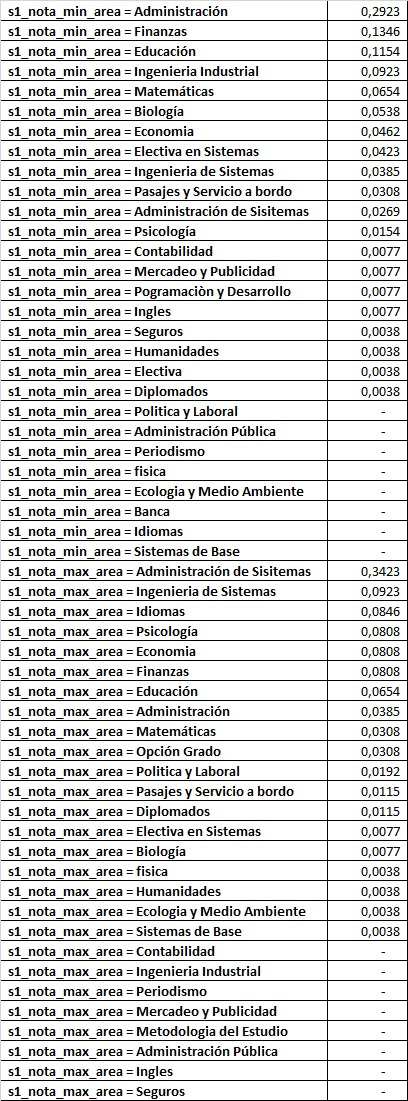
\includegraphics[width=8cm]{img/cluster-s1.jpg}\\ 

\subsection{Clustering de desertores en segundo semestre}

Para los desertores en segundo semestre se realizaron las mismas tareas de preparación de datos, incluyendo las nuevas columnas correspondientes a información de segundo semestre.\\

En este segundo ejercicio de clustering, se realizó la misma tarea de observación encontrando lo que sigue:\\

{\bf \textbullet\ Cluster 1:}\\

\begin{itemize}
	\item No perdieron materias en primer semestre.
	\item En segundo semestre perdieron entre 3 y 4 materias.
	\item Promedio general primer semestre: 3.8.
	\item Promedio general segundo semestre: 2.4.
	\item Promedio general nota mínima primer semestre: 3.2.
	\item Promedio general nota máxima primer semestre: 4.4.
	\item Promedio general nota mínima segundo semestre: 1.1.
	\item Promedio general nota máxima segundo semestre: 3.7.
	\item Tendencias de edad: 47.8\% total mayores de 31, y 64\% total mayores de 28.
	\item 67\% de notas mínimas primer semestre en materias de matemáticas, educación y contabilidad.
	\item 60\% de notas máximas primer semestre en materias de administración de sistemas y matemáticas.
	\item 63\% de notas mínimas segundo semestre en materias de matemáticas, ingeniería industrial, administración y contabilidad.
	\item 61\% de notas máximas segundo semestre en materias de Política, contabilidad, administración y humanidades.
\end{itemize} 

{\bf \textbullet\ Cluster 2:}\\

\begin{itemize}
	\item No perdieron materias en primer semestre.
	\item No perdieron materias en segundo semestre.
	\item Promedio general primer semestre: 3.9.
	\item Promedio general segundo semestre: 3.9.
	\item Cantidad de materias inscritas primer semestre: 10.2 (Homologaciones de otras instituciones).
	\item Promedio general nota mínima primer semestre: 3.3.
	\item Promedio general nota máxima primer semestre: 4.5.
	\item Promedio general nota mínima segundo semestre: 3.4.
	\item Promedio general nota máxima segundo semestre: 4.5.
	\item 60\% de notas mínimas segundo semestre en materias de contabilidad, economía e idiomas.
	\item 63\% de notas máximas segundo semestre en materias de contabilidad, matemáticas, ecología e idiomas.
\end{itemize} 

{\bf \textbullet\ Cluster 0:}\\

\begin{itemize}
	\item Perdieron 70\% de materias en primer semestre.
	\item No perdieron materias en segundo semestre.
	\item Inscribieron 8 materias en primer semestre (homologaciones).
	\item Idiomas como nota mínima en el 17\% de los casos, tanto en primer como segundo semestre.
\end{itemize} 

{\bf \textbullet\ Cluster 4:}\\

\begin{itemize}
	\item Perdieron todas (o casi todas en su gran mayoría) las materias en primer semestre.
	\item Perdieron todas las materias en segundo semestre.
	\item Nota mínima en primer semestre: 0.9.
	\item Nota máxima en primer semestre: 3.1.
	\item Nota mínima en primer semestre: 0.15.
	\item Nota máxima en primer semestre: 1.1.
\end{itemize}

\subsection{Clustering de desertores en tercer semestre}

Para los marcados como desertores en tercer semestre se identificaron los siguientes grupos especiales:

{\bf \textbullet\ Cluster 0:}\\

\begin{itemize}
	\item Perdieron en promedio 2 a 3 materias en primer semestre
	\item Perdieron en promedio 4 a 5 materias en segundo semestre
	\item Perdieron en promedio 2 materias en tercer semestre
	\item Promedio primer semestre: 3.1
	\item Promedio segundo semestre: 2.2
	\item Promedio tercer semestre: 2.8
	\item Cantidad de estudiantes repartidos proporcionalmente en las categorías de edad
	\item 28\% de notas mínimas primer semestre en materias de matemáticas
	\item 35\% de notas mínimas segundo semestre en materias de matemáticas
	\item 11\% de notas mínimas segundo semestre en materias de inglés
	\item 36\% de notas mínimas tercer semestre en materias de matemáticas
\end{itemize}

{\bf \textbullet\ Cluster 1:}\\
 
\begin{itemize}
	\item En promedio perdieron 0 o 1 materias en cada semestre de los tres semestres cursados
	\item 100\% Mayores de 33 años
\end{itemize}

{\bf \textbullet\ Cluster 4:}\\

\begin{itemize}
	\item Perdieron en promedio 3 materias en primer semestre
	\item Perdieron en promedio 5 materias en segundo semestre
	\item Perdieron en promedio 5 materias en tercer semestre
	\item 51\% de notas mínimas segundo semestre en materias de matemáticas y economía
	\item 30\% de notas mínimas segundo semestre en materias de economía
\end{itemize}


\subsection{Conclusiones}

Con base en los resultados encontrados en el ejercicio de clustering expuesto anteriormente, las conclusiones a las que podemos llegar son las siguientes:

\begin{itemize}
	\item Los estudiantes con edades mayores tienden a desertar, independiente de los resultados académicos que obtengan.
	\item Los estudiantes que llegan de otras instituciones y pierden varias materias, tienden a desertar más seguido.
	\item Las materias de las áreas de economía y matemáticas estimulan un alto grado de deserción en el tercer semestre.
	\item Los estudiantes mayores de 28 años que pierden más de 3 materias en segundo semestre, tienen una mayor tendencia a la deserción.
\end{itemize}

\subsection{Mejoras y trabajos futuros}

En primera instancia, hubiera sido mucho más útil contar con mayor información demográfica de los estudiantes, con el fin de detectar patrones de deserción relacionados con dicha información.; por ejemplo, hubiese sido interesante encontrar los grupos de deserción, relacionando información de sexo, estrato, lugar de vivienda, etc.

Por otra parte, encontramos que se podrían realizar otro tipo de detecciones de grupos naturales, pero teniendo en cuenta otras variables que no se descubrieron al inicio del proyecto, tales como homologación de materias cuando los estudiantes vienen de otras instituciones, o tendencias de cumplimiento de pago de matrículas.



%----------------------------------------------------------------------------------------
%	REFERENCE LIST
%----------------------------------------------------------------------------------------
\phantomsection
\bibliographystyle{unsrt}
\bibliography{sample}

%----------------------------------------------------------------------------------------

\end{document}

% Ejemplo de agregar algo a la tabla de contenido
% \addcontentsline{toc}{section}{Introducción} % Adds this section to the table of contents

% Ejemplo de tabla

%\begin{table}[hbt]
%\caption{Table of Grades}
%\centering
%\begin{tabular}{llr}
%\toprule
%\multicolumn{2}{c}{Name} \\
%\cmidrule(r){1-2}
%First name & Last Name & Grade \\
%\midrule
%John & Doe & $7.5$ \\
%Richard & Miles & $2$ \\
%\bottomrule
%\end{tabular}
%\label{tab:label}
%\end{table}

% Ejemplo de imagen

%\begin{figure*}[ht]\centering % Using \begin{figure*} makes the figure take up the entire width of the page
%\includegraphics[width=\linewidth]{view}
%\caption{Wide Picture}
%\label{fig:view}
%\end{figure*}

% Ejemplo de ecuación

%\begin{equation}
%\cos^3 \theta =\frac{1}{4}\cos\theta+\frac{3}{4}\cos 3\theta
%\label{eq:refname2}
%\end{equation}

% Ejemplo de enumeración

%\begin{enumerate}[noitemsep] % [noitemsep] removes whitespace between the items for a compact look

%\item First item in a list
%\item Second item in a list
%\item Third item in a list
%\end{enumerate}

% Ejemplo de viñetas

%\begin{itemize}[noitemsep] % [noitemsep] removes whitespace between the items for a compact look
%\item First item in a list
%\item Second item in a list
%\item Third item in a list
%\end{itemize}


% Ejemplo de referencia a figura

%Reference to Figure \ref{fig:results}.


% Ejemplo de descripción, concepto o idea

%\begin{description}
%\item[Word] Definition
%\item[Concept] Explanation
%\item[Idea] Text
%\end{description}
